\documentclass[a4paper,10pt,twocolumn,uplatex]{jsarticle}
\usepackage{style/nislab}

%---------------------------------------------------------------------
% レジュメ種別・日付設定(要変更)
% \type{} 1:修士論文諮問会 2:卒業論文発表会 else:月例発表会
\type{3}
\year{2021}
\month{7}
\date{10}

%---------------------------------------------------------------------
% ページ番号設定(要変更)
\setcounter{page}{9}

%---------------------------------------------------------------------
\begin{document}
%---------------------------------------------------------------------
% タイトル作成部分(要変更)
% \maketitle{タイトル}{title}{名前}{name}
\maketitle{スマートホームにおけるSDNを用いたトラフィック監視による不正アクセス防御手法の検討}
{A Study on Unauthorized Access Protection Method by Traffic Monitoring Using SDN in Smart Home}
{塚﨑 拓真}
{Takuma Tsukasaki}

%---------------------------------------------------------------------
\section{はじめに}
近年,IoT(Internet of Things)が注目を集めるようになり,今後あらゆるものがネットワークに接続され,利用されることが予想される.
現在,IoT機器が様々なところに置かれるようになり,以前のパソコンやスマートフォンに限らず,現在ではテレビやゲーム機,Webカメラ,冷蔵庫などの家電などがインターネットに繋がり,情報を通信するようになっている.
それに伴い,ネットワークないには様々な端末や機器が混在することになる.ホームネットワークは情報家電などの普及も加わり,その形態が多様化していくと考えられる.\par
しかし,IoTの登場で利便性が高まる一方で,これまでのネットワークに接続されていないモノが接続されることにより,セキュリティ上のリスクが高まっている\cite{guideline}.
IoTはセキュリティを考慮せずに開発されたものが多く、悪意のある攻撃者によるサイバー攻撃の標的になりやすく,特に不正アクセスが多発している.
これらが各種端末やネットワークごとに顕在した場合、個別に対処するとコストや時間がかかってしまうため、脅威に対し一括に対処する必要がある.
ホームネットワーク内には異なる規格のハードウェアやそれらに搭載される様々なアプリケーションが混在しているため、それら全てに対応したシステムの構築や更新を続けるのは困難である.
ホームネットワーク内には異なる規格のハードウェアやそれに対応したソフトウェアとして構築するのではなく、ホームネットワーク内で通信するのであれば、どの端末も必ず利用するネットワークを利用したシステムを構築することが望ましい.

%---------------------------------------------------------------------
\section{関連研究}
村上らは,OpenFlowを用いてホームネットワーク内に、動的な認証システムを構築し、不正アクセスによる被害を軽減する手法を提案した。
本提案方式では、認証時に頻繁に利用される情報を用いることで、ネットワークに接続する端末を制限すると共に、万が一認証が突破された場合でも不正アクセスが検出できるシステムを構築した。
しかし、1度入られてしまったら、攻撃されてしまう。
現在のスマートホームデバイスは、クラウド上のシステムと連携することで、デバイス間の連携を可能にしているが、今後はホームネットワーク内で閉じたデバイス間の通信によって連携を行う形になることが想定される\cite{d2d}。
また、同じホームネットワークに他の多くの機器が何の制限もなく接続されているという事実を利用して、マルウェアをインストールする。
カメラに搭載されたマルウェアは、ローカルネットワーク上で他の潜在的に脆弱なデバイスをスキャンし、例えばよく知られたセキュリティ上の欠陥を利用してそれらのデバイスにアクセスし、同じまたは異なるマルウェアのコピーをさらにインストールしようとする。
感染した機器がマルウェアの支配下に置かれると、個人情報の漏洩など、スマートホームネットワーク自体に被害を及ぼすだけでなく、DDoS攻撃への加担やサービスの操作など、他の悪意ある活動を行う可能性がある\cite{disap}。

%---------------------------------------------------------------------
\subsection{図}
図を挿入する場合は,図\ref{fig:sample1}や\figref{fig:sample2}のように引用することができる.図の横幅が大きい場合は,\figref{fig:sample2}のようにすることもできる.\par
ちなみに,\LaTeX{}ではベクターファイルとしてEPSファイルを推奨していた頃もあったようだが,現在はPDFファイルを使用することが推奨されている.PDFファイルに出力するのが前提なら,dvipdfmxではPDF,PNG,JPEG がそのまま使用できる.dvipdfmxはEPSファイルそのものを自分で扱えないので,Ghostscriptを内部で呼び出して変換する.PDFファイルで問題がなければEPSにこだわる必要はないと思われる.ただし,ジャーナルによっては図としてPDFを使うのがダメだったりするので慎重に.

\begin{figure}[!tb]
  \centering
  
\includegraphics[width=\linewidth]{img/sample1.pdf}
  \caption{悩む男の子}
  \label{fig:sample1}
\end{figure}

\begin{figure*}[!tb]
  \centering
  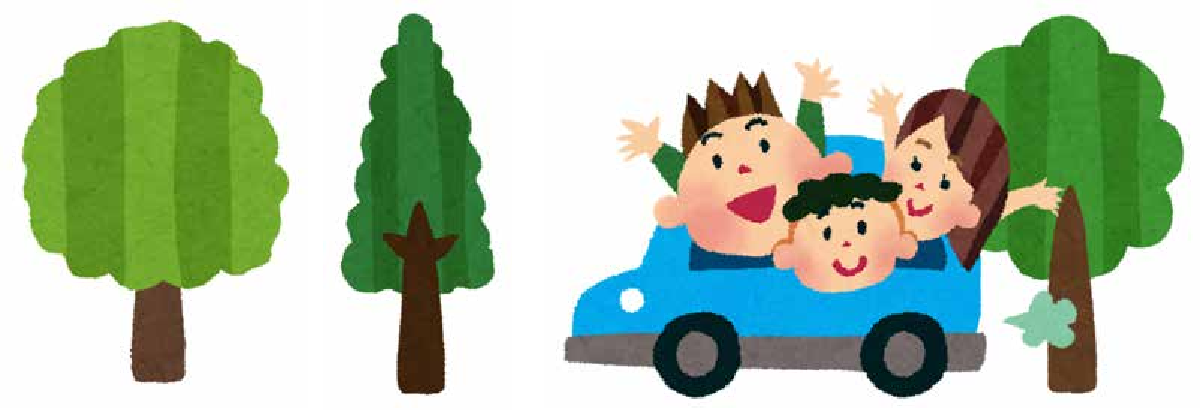
\includegraphics[width=\linewidth]{img/sample2.pdf}
  \caption{ドライブする家族}
  \label{fig:sample2}
\end{figure*}

%---------------------------------------------------------------------
\subsection{表}
表は\tabref{tab:data_type}のように引用することができ,表を作成する場合は罫線を少なくすることと,横線のみの使用を心がけることが推奨される.

\begin{table}[!bt]
  \caption{代表的なデータの型}
  \label{tab:data_type}
  \centering
  \begin{tabular}{lcr}
    \hline
    データの型         & 宣言   & ビット幅 \\
    \hline \hline
    短整数型           & short  & 16       \\
    整数型             & int    & 32       \\
    単精度浮動小数点型 & float  & 32       \\
    倍精度浮動小数店型 & double & 64       \\
    \hline
  \end{tabular}
\end{table}

%---------------------------------------------------------------------
\section{研究者にとっての論文十箇条}
論文を書くことは大切だ必要だ,と周囲から言われる.それは自分でも分かっているつもりだけれど,その理由をはっきりと伝えてもらえる機会は少ない.研究者にとっての論文十箇条\cite{whats_paper}は,とてもシンプルでわかりやすく,非常に心にきた.一度目を通してみるべきであろう.

\begin{enumerate} % 箇条書きは \begin{itemize}
  \item 書かれた論文は書いた人の研究者としての人格を表す
  \item データのみ出して論文を書かない者は,テクニシャンである
  \item データも出さず,論文(原著論文)を書かない者は,評論家である
  \item 研究者は論文を書くことによって成長する.また,成長の糧にしなければならない
  \item 論文は研究者の飯のタネである
  \item 論文は後世の研究に影響を与えなければならない
  \item 研究者は書いた論文に責任を問われる
  \item 忙しくて論文が書けないというのは,言い訳にはならず,能力がないといっているのと同じである
  \item 博士論文以上の論文を書けない者は,その博士論文は指導教官のものといわれても仕方がない
  \item 研究において最も重要なのはアイデアであり,それが試されるのが論文である
\end{enumerate}

%---------------------------------------------------------------------
% Bibliography
\footnotesize{
  \begin{thebibliography}{99}
    \bibitem{guideline} IoT推進コンソーシアム, 総務省, 経済産業省, "IoTセキュリティガイドライン ver 1.0", 2016.
    \bibitem{d2d} C. Vallati, A. Virdis, E. Mingozzi and G. Stea, "Mobile-Edge Computing Come Home Connecting things in future smart homes using LTE device-to-device communications," IEEE Consumer Electronics Magazine, Vol.5, No.4, pp. 77-83, 2016.
    \bibitem{disap} M. Serror, M. Henze, S. Hack, M. Schuba, and K. Wehrle, "Towards In-Network Security for Smart Homes," Proceedings of the 13th International Conference on Availability, Reliability and Security (ARES 2018), No.18, pp.1–8, 2018.
  \end{thebibliography}
}

%---------------------------------------------------------------------
\end{document}
%---------------------------------------------------------------------
